\begin{frame}%[plain, noframenumbering, t]
    \frametitle{Проблемная ситуация}

    При создании прикладного ПО для специализированного аппаратного обеспечения
    дорого обеспечивать разработчиков самим аппаратным обеспечением.

    \textbf{Причины сложившейся ситуации:}
    \begin{itemize}
        \item печать экземпляров аппаратного обеспечения в условиях санкций и дефицита полупроводников стала дорогой;
        \item простаивание программистов, пока происходит печать и доставка аппаратного обеспечения;
        \item трудоемкость создания собственного виртуального аппаратного обеспечения.
    \end{itemize}
\end{frame}


\begin{frame}%[plain, noframenumbering, t]
    \frametitle{Цель и задачи диссертации}
    \textbf{Цель:} снижение трудоемкости создания виртуальных устройств.

    \textbf{Задачи:}
    \begin{itemize}
        \item аналитический обзор существующих методов создания виртуального аппаратного обеспечения;
        \item формализация задачи;
        \item создание методики и алгоритма генерации виртуального аппаратного обеспечения на основе его спецификации;
        \item разработка лингвистического аппарата (семантика, синтаксис) языка для создания программ по генерации виртуального
            аппаратного обеспечения.
    \end{itemize}
\end{frame}


\begin{frame}%[plain, noframenumbering, t]
    \frametitle{Положения, выносимые на защиту}
    \begin{itemize}
        \item формализованное представление алгоритма генерации виртуального аппаратного обеспечения;
        \item лингвистический аппарат (синтаксис, семантика) языка для создания программ по генерации виртуального
            аппаратного обеспечения;
        \item экспериментальные результаты применения генератора аппаратного обеспечения.
    \end{itemize}
\end{frame}


\begin{frame}%[plain, noframenumbering, t]
    \frametitle{Анализ существующих методов создания виртуального аппаратного обеспечения}
    \newcommand{\tabitem}{{\textbullet}~}
        {\scriptsize
            \begin{longtable}{| p{3cm} | p{3cm} | p{4cm} |}
                \hline
                Метод & Особенности & Недостатки \\
                \hline
                    Создание stub-симулятора &
                    Требует создания интерфейсов-адапторов в прикладном ПО &
                    Приходится создавать интерфейсы-адапторы для каждого разрабатываемого ПО \\
                \hline
                    Использование записи работы аппаратного обеспечения &
                    Быстрый метод, не требует специальных знаний о внутреннем устройстве аппаратного обеспечения &
                    \tabitem Взаимодействие ПО с аппаратным обеспечением ограничивается заранее записанными сценариями \\
                \makecell{} & \makecell{} & \tabitem Количество записей очень быстро разрастается \\
                \makecell{} & \makecell{} & \tabitem Зачастую записи снимаются только с корректных сценариев использования \\
                \hline
                Использование эмулятора QEMU &
                \tabitem Готовая инфраструктура для создания виртуального аппаратного обеспечения &
                \tabitem Необходимость написания виртуального аппаратного обеспечения на низкоуровневом языке \\
                \makecell{} &
                \tabitem Постоянная поддержка эмулятора силами сообщества &
                \tabitem Необходимость обучения объектной системе QEMU (QOM) \\
                \hline
            \end{longtable}
        }
\end{frame}


\begin{frame}%[plain, noframenumbering, t]
    \frametitle{Формализованное представление (грамматика)}
    \begin{figure}[!htbp]
        \begin{adjustbox}{max totalsize={\textwidth}{\textheight}}
            \begin{minipage}{\linewidth}
                {\footnotesize
                \setlength{\grammarparsep}{0.02cm}
                \setlength{\grammarindent}{13em}
                \begin{grammar}{}
                    <letter> ::= `a' ... `z' | `A' ... `Z';

                    <digit> ::= `0' ... `9' ;

                    <symbol> ::= \symbol{92}x20 ... \symbol{92}x7E ; (* любой печатный символ, согласно кодам ASCII *)

                    <const value> ::= <digit> | `"' \{ <symbol> \} `"';

                    <identifier> ::= <letter> [\{ <letter> | <digit> | `\_' \}] ;

                    <block start> ::= `{';

                    <block end> ::= `}';

                    <field> ::= <identifier> `=' <identifier> | <block> ;

                    <block> ::= <block start> <field> [\{ `,' <field> \}] <block end>;

                    <device definition> ::= '\#' <identifier>;

                    <device class inheritance> ::= `(' <identifier> `:' <identifier> [\{ `,' <identifier> \}] `)';

                    <device class block> ::= <device class inheritance> <block>;

                    <bind block> ::= `@bind' <block>;

                    <python block> ::= `@py' <block>;

                    <program> ::= <device definition> <device class block> <bind block> <python block>;
                \end{grammar}
                }
            \end{minipage}
        \end{adjustbox}
        \caption{Расширенная форма Бэкуса-Наура генератора виртуального аппаратного обеспечения}
    \end{figure}
\end{frame}


\begin{frame}%[plain, noframenumbering, t]
    \frametitle{Формализованное представление (семантика)}
    \begin{figure}[!htbp]
        \begin{adjustbox}{max totalsize={\textwidth}{\textheight}}
        \begin{minipage}{\linewidth}
                \centering
                \begingroup
                \begin{align*}
                    [[assignment]](x,y) ={}& \lambda x.y \\
                    [[terminate]](m) ={}& \text{ Завершение работы компилятора} \\
                    [[if]](c,e_1,e_2) ={}&
                    \begin{cases}
                        e_1, & \text{Если } c = true \\
                        e_2, & \text{Если } c \not= true
                    \end{cases} \\
                    [[throw\ error]](c, e) ={}& if(c, e_g, terminate) \\
                    [[lookup]](o) ={}& [[throw\ error]](o \in Q, o) \\
                    [[<device\ definition>]](i) ={}& lookup(i) \\
                    [[<device\ class\ inheritance>]](i_1,...,i_n) ={}& lookup(i_1) + ... + lookup(i_n) \\
                    [[<field>]](v_1, v_2) ={}& assignment(v_1, v_2), \text{ Если } v_1 \in Q \text{ и } v_3 \in C \cup Q \\
                    [[<block>]](f_1,...,f_n) ={}& field(f_1) + ... + field(f_n) \\
                    [[<python block>]](b) ={}& assignment(B,B)\\
                \end{align*}
                \endgroup
            \end{minipage}
        \end{adjustbox}
        \caption{Денотационная семантика генератора виртуального аппаратного обеспечения}
    \end{figure}
\end{frame}%[plain, noframenumbering, t]


\begin{frame}%[plain, noframenumbering, t]
    \frametitle{Методика создания виртуального аппаратного обеспечения}
    \begin{figure}[!htbp]
        \centering
        \begin{adjustbox}{max totalsize={\textwidth}{\textheight}}
            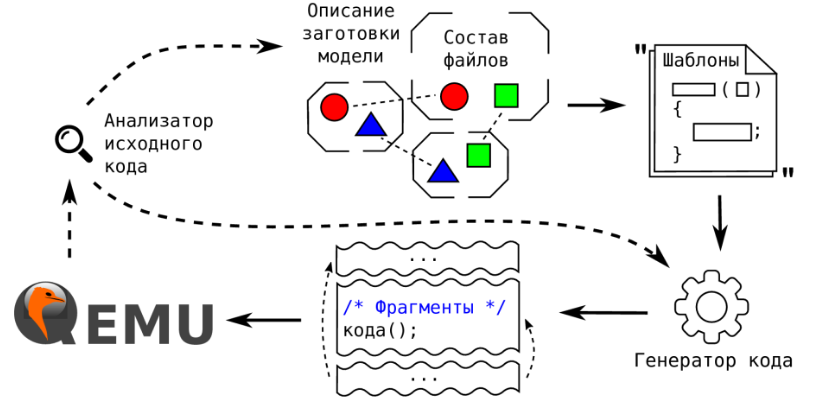
\includegraphics[]{images/imposter_algorithm.png}
        \end{adjustbox}
    \end{figure}
\end{frame}


\begin{frame}%[plain, noframenumbering, t]
    \frametitle{Выбор метрики оценки эффективности}
    Основные метрики эффективности:
    \begin{itemize}
        \item время разработки виртуального устройства (в человеко-часах);
        \item быстродействие сгенерированного виртуального аппаратного обеспечения.
    \end{itemize}
\end{frame}


\begin{frame}%[plain, noframenumbering, t]
    \frametitle{Основные результаты диссертационной работы}
    \begin{itemize}
        \item проведен аналитический обзор существующих методов создания виртуального аппаратного обеспечения;
        \item созданы методика и алгоритм генерации виртуального аппаратного обеспечения на основе его спецификации;
        \item разработан лингвистический аппарат (семантика, синтаксис) языка для создания программ по генерации виртуального
            аппаратного обеспечения;
    \end{itemize}
\end{frame}


\begin{frame}%[plain, noframenumbering, t]
    \begin{center}
        \Huge Спасибо за внимание!
    \end{center}
\end{frame}
